\begin{center}
    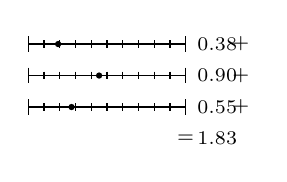
\begin{tikzpicture}
        \foreach \y in {0, -0.4, -0.8} {
            \draw (0, \y) -- (2, \y);

            \draw (0, \y + 0.1) -- (0, \y - 0.1);
            \draw (2, \y + 0.1) -- (2, \y - 0.1);
            \foreach \x in {0.2, 0.4, ..., 1.8} {
                \draw (\x, \y + 0.05) -- (\x, \y - 0.05);
            }
        }

        \fill (0.38, 0) circle (0.04);
        \fill (0.9, -0.4) circle (0.04);
        \fill (0.55, -0.8) circle (0.04);

        \node at (2.4, 0) {\scriptsize \( 0.38 \)};
        \node at (2.4, -0.4) {\scriptsize \( 0.90 \)};
        \node at (2.4, -0.8) {\scriptsize \( 0.55 \)};

        \node at (2.7, 0) {\scriptsize \( + \)};
        \node at (2.7, -0.4) {\scriptsize \( + \)};
        \node at (2.7, -0.8) {\scriptsize \( + \)};

        \node at (2.4, -1.2) {\scriptsize \( 1.83 \)};
        \node at (2.0, -1.2) {\scriptsize \( = \)};
    \end{tikzpicture}
\end{center}
\captionof{figure}{One realization of the state of the sliders and their sum for \( n = 3 \). We see that this state is included in the set of solutions for which the sum is greater than \( 1 \).}
